\documentclass[a4paper]{exam}
\usepackage[english]{babel}
\usepackage[fleqn]{amsmath}
\usepackage{amsthm}
\usepackage{amssymb}
\usepackage{amsmath}
\usepackage{mathtools}
\usepackage{enumerate}
\usepackage{tabstackengine}
\usepackage{thmtools}
\usepackage{xcolor}
\usepackage[bookmarks=true, hidelinks]{hyperref}
\usepackage{bookmark}
\usepackage{pdfpages}

\makeatletter
\renewcommand\@seccntformat[1]{}
\makeatother

\theoremstyle{definition}
\newtheorem*{define}{Definitie}
\newtheorem*{theorem}{Stelling}
\newtheorem*{lemma}{Lemma}
\newtheorem*{opm}{Opmerking}
\newtheorem*{gevolg}{Gevolg}
\newtheorem*{nota}{Notatie}
\newtheorem*{valkuil}{\textcolor{red}{Valkuil}}
\newtheorem*{note}{\textcolor{red}{Note}}

\DeclareMathOperator{\intr}{int}
\DeclareMathOperator{\dist}{dist}

%--------------------Make usable space all of page
\setlength{\oddsidemargin}{0in}
\setlength{\evensidemargin}{0in}
\setlength{\topmargin}{0in}
\setlength{\headsep}{-.25in}
\setlength{\textwidth}{6.5in}
\setlength{\textheight}{8.5in}

%--------------------Indention
\newlength\tindent
\setlength{\tindent}{\parindent}
\setlength{\parindent}{0pt}
\renewcommand{\indent}{\hspace*{\tindent}}

\stackMath
\makeatletter\renewcommand\TAB@delim[1]{\displaystyle#1}\makeatother
\setstackEOL{\cr}% ROW DELIMITER FOR STACKS
\renewcommand\stackalignment{l}% LEFT ALIGNMENT OF STACKS
\setstackgap{S}{8pt}% INTER-ROW PADDING OF SHORT STACKS

% Number sets
\newcommand{\naturals}{\mathbb{N}}
\newcommand{\reals}{\mathbb{R}}
\newcommand{\complex}{\mathbb{C}}
\newcommand{\rationals}{\mathbb{Q}}

\begin{document}
\section{College 15}
    \subsection{Eigenschappen van de norm}
    \begin{enumerate}[(i)]
      \item \Longunderstack{\forall x\in \mathbb{R}^d:|x| \geq 0 \cr |x|=0 \Leftrightarrow x=0}
      \item $|cx|=|c||x|$ ($|$norm$|$ = $|$absolute waarde$||$norm$|$)
      \item ongelijkheid van \textbf{Cauchy-Schwartz}
        \[\forall x,y \in \mathbb{R}^d: \sum_{i=1}^{d}x_i y_i = (x,y)\]
        \[|(x,y)| \leq |x||y|\]
      \item driehoeksongelijkheid
        \[\forall x,y \in \mathbb{R}^d: |x+y|\leq |x|+|y|\]
    \end{enumerate}
    \subsection{Afstand in $\mathbb{R}^d$ $\dist(x,y):=|x-y|$}
        Eigenschappen:
            \begin{align*}
              |x-y| & \geq 0 \\
              |x-y| & =0 \Leftrightarrow x=y \\
              |x-y| & \leq |x-z| + |z-y|
            \end{align*}
        \define Zij $x \in \mathbb{R}^d, R>0$.
              $B(x,r)={y \in \mathbb{R}^d | |y-x|<r }$ (open) \underline{bol} rond $x$ met straal $r$.
		\define Zij $x \in \mathbb{R}^d, A \subset \mathbb{R}^d$. $x$ heet \textbf{inwendig punt} (\textit{interior point}) van $A$ als $\exists _{r>0}:B(x,r) \subset A$. $A$ heet dan een \textbf{omgeving} (\textit{neighbourhood}) van $x$.

              \textbf{Inwendige van $A$, open kern van $A$}
              \[\intr A=\AA=\big\{x \in A \bigm| x \text{ inwendig punt van } A\big\}\]
              $A$ heet \textbf{open verzameling} als $A=\AA$, oftewel: $\forall _{x \in A} \exists _{R \in (0,\infty)}: B(x,R) \subset A$, oftewel elk punt van $A$ is een inwendig punt.
        \theorem
          \begin{enumerate}[(1)]
                \item Zij $\big\{A_\alpha \bigm| \alpha \in I \big\}$ een familie van open verzamelingen $A_\alpha \subset \mathbb{R}^d$. Dan $\bigcup_{\alpha \in I}A_\alpha$ open.
                \item Zij $A_1,A_2,\dots,A_n \in \mathbb{R}^d$ open. Dan $\bigcap_{i=1}^{n}A_i$ open.
          \end{enumerate}

        \theorem
          \begin{enumerate}[(i)]
            \item $\intr A=\bigcup_{C \subset A, C \text{ open} }C=\bigcup \big\{C \bigm| C \subset A, C \text{ open} \big\}$
            \item $\intr A$ open. Volgt uit $(i)$ en 10.1.4
          \end{enumerate}

        \define \textbf{Rand van $A \subset \mathbb{R}^d$}
            \[\partial A:= \mathbb{R}^d\backslash (\intr A \cup \intr (\mathbb{R}^d\backslash A))\]
              d.w.z: $x$ is een randpunt van $A \Leftrightarrow x$ geen inwendig punt van $A$ en geen inwendig punt van het complement $\mathbb{R}^d\backslash A$.

        \lemma
        	Elke $x \in \mathbb{R}$ hoort precies 1 van de drie verzamelingen $\intr A, \intr (\mathbb{R}^d\backslash A), \partial A$.

  	\subsection{Stellingen uit het huiswerk}
        \theorem $x \in \mathbb{R}^d, r>0$, dan $B(x,r) open$.
\newpage
\section{College 16}
	\subsection{Convergentie in $\mathbb{R}^d$}
		\define Zij $(\underline{x}^{(n)}) = ((x^{(1)},\dots ,x^{(1)}),(x^{(2)},\dots ,x^{(2)}),\dots )$ een rij in $\mathbb{R}^d$, en $\underline{a}=(a_1, \dots ,a_d ) \in \mathbb{R}^d$. $(x^{(n)}) $ heet convergent naar $\underline{a}$ als
			\begin{enumerate}[(i)]
				\item $|x^{(n)}-a|\stackrel{n\rightarrow \infty}{\longrightarrow} 0$
				\item $\forall _{\varepsilon >0} \exists _{n_0=n_0(\varepsilon)}: \forall _{n\geq n_0} : |x^{(n)} - a| < \varepsilon$.
				\item $\forall _{\varepsilon >0} \exists _{n_0=n_0(\varepsilon)}: \forall _{n\geq n_0} : x^n \in B(a,\varepsilon )$
			\end{enumerate}
		
		\theorem $\lim_{n\rightarrow\infty}\underline{x}^{(n)}=\underline{a} \Leftrightarrow \lim_{n\rightarrow\infty} x_{i}^{(n)} = a_i$ voor $i=1,\dots ,d$.
		
		\define Zij $A \subset \mathbb{R}^d$. Een punt $x \in \mathbb{R}^d$ heet \textbf{verdichtingspunt} van $A$ als \[\forall _{R>0}:B(x,R)\cap  A \backslash\{x\} \neq \emptyset.\]
			Dan $A':=\big\{ x \in \mathbb{R}^d \bigm| x \text{ verdichtingspunt van } A\big\}$.
		
		\lemma Zij $A \subset \mathbb{R}^d$. Dan $\partial A \subset A\cup A'$.
		\define $A \subset \mathbb{R}^d$ heet \textbf{gesloten} als haar \underline{complement open} is.
		\valkuil Een niet open/gesloten verzameling is in het algemeen niet gesloten/open.
		
		\theorem[Karakterisering voor geslotenheid] Zij $A \subset \mathbb{R}^d$. De volgende beweringen zijn equivalent:
			\begin{enumerate}[(i)]
				\item $A$ gesloten
				\item $A'\subset A$
				\item $\partial A \subset A$
				\item voor elke convergente rij in $A$ ligt de limiet in $A$. (limiet convergente rij blijft in $A$)
			\end{enumerate}
		
		\theorem $\left[\text{K}\right]$ 10.1.6
			\begin{enumerate}[(i)]
				\item Zij $\big\{ A_\alpha \bigm| \alpha \in I \big\}$ een familie gesloten verzamelingen $A_\alpha \subset \mathbb{R}^d$. Dan $\bigcap_{\alpha \in I}A_\alpha$ gesloten.
				\item Zij $A_1, \dots ,A_n$ gesloten. Dan $\bigcup_{i=1}^n A_i$ gesloten.
			\end{enumerate}
		
		\define Zij $A \subset \mathbb{R}^d$. De verzameling $\overline{A}:= \mathbb{R}^d \backslash (\intr (\mathbb{R}^d \backslash A))$ heet de \textbf{afsluiting} (\textit{closure}) van $A$.
		\theorem[Karakterisering voor de afsluiting]
			  Zij $A \subset \mathbb{R}^d$. Dan
			\[\overline{A}= A \cup \partial A = A \cup A'= \big\{z \in \mathbb{R}^d \bigm| \exists _{\text{rij } (x^{(n)}) \text{ in } A \text{ met } x^{(n)} \rightarrow z} \big\}\]
	
	\subsection{Stellingen uit het huiswerk}
		\theorem Zij $(x^{(n)})$ een rij in $\mathbb{R}^d, a \in \mathbb{R}^d$. Dan $x^{(n)}\rightarrow a \Rightarrow |x^{(n)}|\rightarrow |a|.$
		\theorem Zij $z \in \mathbb{R}^d, A \subset \mathbb{R}^d, A \neq \emptyset, \text{dist}(z,A) := \text{inf}_{x\in A}|x-z|$.
		  Dan $\overline{A}=\big\{z\in \mathbb{R}^d \bigm| \text{dist}(z,A)=0\big\}$.
\newpage
\section{College 17}
	\subsection{Compacte verzamelingen in $\mathbb{R}^d$}
		\define Een verzameling binnen $\mathbb{R}^d$ heet \textbf{begrensd} als \[\exists _{R>0}: A \subset B(0,R)\]
		\[\forall _{x\in A}: \|x\|<R.\]
		
		\theorem $\left[\text{K}\right]$ 10.1.7 (andere formulering)
			  Zij $A \subset \mathbb{R}^d$. De volgende beweringen zijn equivalent:
			\begin{enumerate}[(i)]
				\item Elke rij $x^{(n)}$ in $A$ heeft een convergente deelrij met limiet $x^* \in A$.
				\item $A$ begrensd en gesloten
			\end{enumerate}
		
		\define Zij $K \subset \mathbb{R}^d$. Een familie $\big\{A_\alpha \bigm| \alpha \in I \big\}$ van verzamelingen $A_\alpha \subset \mathbb{R}^d$ heet een \textbf{overdekking} (\textit{cover, covering}) van $K$ als \[K \subset \bigcup_{\alpha \in I}A_\alpha\]
		
		\begin{itemize}
			\item Een overdekking $\big\{ A_\alpha \bigm| \alpha \in I \big\}$ heet \underline{open} als alle $A_\alpha$ open zijn in $\mathbb{R}^d$.
			\item Een overdekking $\mathcal{B}:=\big\{ A_\beta \bigm| \beta \in J\big\}$ heet een \textbf{deeloverdekking} van $\mathcal{A}:=\big\{ A_\alpha \bigm| \alpha \in I \big\}$ als $\mathcal{B} \subset \mathcal{A}$.
		\end{itemize}
		
		\define $K \subset \mathbb{R}^d$ heet \textbf{compact} als elke open overdekking van $K$ een eindige deeloverdekking bevat.
		\note Niet-lege open verzamelingen zijn NOOIT compact.
		
		\theorem[Heine-Borel]
			Zij $K \subset \mathbb{R}^d$. Dan \[K \text{ compact}\Leftrightarrow K \text{ begrensd en gesloten.}\]
			
		\theorem Zij $A,B$ gesloten, niet leeg, $A\cap B = \emptyset$, $A$ compact.
			  Dan $\text{dist}(A,B) = \text{inf}\big\{ |a-b| \bigm| a \in A, b \in B \big\} > 0$.
			\opm $A \subset \mathbb{R}^d$ relatief compact $\Leftrightarrow \overline{A}$ compact.

	\subsection{Stellingen uit het huiswerk}
		\theorem Zij $A \subset \mathbb{R}^d$. Equivalente beweringen:
			\begin{enumerate}[(i)]
				\item $A$ is begrensd
				\item $\exists _{x \in \mathbb{R}^d} \exists _{R>0}: A \subset B(x,R)$
      			\item $\forall _{x \in \mathbb{R}^d} \exists _{R>0}: A \subset B(x,R)$
      			\item De verzamelingen $\{ x_i | x \in A \}, i=1,\dots,d$ zijn begrensde deelverzamelingen van $\mathbb{R}$
      			\item De verzameling $\big\{|x-y| \bigm| x,y \in A \big\}$ is begrensd.
			\end{enumerate}
		
		\theorem Zij $A \subset \mathbb{R}^d$. Dan \[A \text{ begrensd} \Leftrightarrow \overline{A} \text{ begrensd} \Leftrightarrow \overline{A}\text{ compact}.\]
		
		\theorem Elke Cauchyrij $(x^{(n)})$ in $\mathbb{R}^d$  \[\forall _{\varepsilon >0} \exists _{n_0=n_0(\varepsilon )\in \mathbb{N}}:\forall _{n,m \geq n_0}: |x^{(n)}-x^{(m)}| < \varepsilon.\] is convergent in $\mathbb{R}^d$.
	
\newpage
\section{College 18}
	\subsection{Functies $\mathbb{R}^d \rightarrow \mathbb{R}$: limieten en continu\"iteit}
		Zij $D \subset \mathbb{R}^d, f: D\rightarrow \mathbb{R}, a \in D'$.
		  Beschrijf lokaal gedrag dicht bij $a$:
		\[ \lim_{x\rightarrow a}f(x)=L \Leftrightarrow \forall _{\varepsilon >0} \exists _{\delta >0} \forall _{x \in D}: 0<|x-a|<\delta \Rightarrow |f(x)-L|<\varepsilon\]
		
		\theorem Zij $D \subset \mathbb{R}^d, f:D\rightarrow \mathbb{R}, a \in D', L \in \mathbb{R}$. Dan geldt
		\[ \lim_{x \rightarrow a} f(x)=L \Leftrightarrow \text{voor elke rij } (x^{(n)}) \text{ in } D\backslash\{a\} \text{ met } x^{(n)}\rightarrow a \text{ geldt } f(x^{(n)}) \rightarrow L.\]
		
		\opm $\left[\text{K}\right]$ 10.2.5 limietstellingen analoog aan 1D.
		
		\define Zij $D \subset \mathbb{R}^d, a\in D\cap D',f:D\rightarrow \mathbb{R}$. $f$ heet \textbf{continu bij $a$} als \[\lim_{x\rightarrow a}f(x)=f(a) \text{ oftewel}\]
		\[\forall _{\varepsilon >0} \exists _{\delta >0}: x \in B(a,\delta)\cap D \Rightarrow |f(x)-f(a)|<\varepsilon.\]
		
		\theorem $\left[\text{K}\right]$ 10.2.7
			  $f$ continu bij $a \Leftrightarrow$ voor elke rij $(x^{(n)})$ in $D: x^{(n)}\rightarrow a \Rightarrow f(x^{(n)}) \rightarrow f(a).$
		
		\theorem Behoud van continu\"iteit
			  $D \subset \mathbb{R}^d, a \in D\cap D', f,g:D\rightarrow \mathbb{R}$, beide continu bij $a$. $0 \not \in R(g)$.
			  Dan $f+g, fg, \frac{f}{g}$ continu bij $a$.
		
        \textbf{Algemener.} Vectorwaardige functies
		  Zij $D \subset \mathbb{R}^d, f:D\rightarrow \mathbb{R}^m, m \in \mathbb{N}_+$. Dat wil zeggen
		\[f(x)=f(x_1,\dots , x_d) =
				\begin{bmatrix}
					f_1(x_1,\dots , x_d) \\
					\vdots \\
					f_m(x_1,\dots , x_d) \\
				\end{bmatrix}, f_i:D\rightarrow \mathbb{R}.\]
				
		\define Zij $a \in D'$.
			\begin{align*}
				\lim_{x\rightarrow a}f(x)=L \in \mathbb{R}^m  &\Leftrightarrow \lim_{x\rightarrow a}f_i(x)=L_i (i=1,\dots ,m) \\
				&\Leftrightarrow \forall _{\varepsilon >0} \exists _{\delta >0}: 0<|x-a|<\delta, x\in D \Rightarrow |f(x)-L|<\varepsilon.
			\end{align*}
		
		\define Zij $a \in D \cap D'$.
		  $f$ heet \textbf{continu} bij $a$:
		\begin{align*}
			\forall _{\varepsilon >0} \exists _{\delta >0}: x\in B(a,\delta) &\Rightarrow |f(x)-f(a)|<\varepsilon \\
			&\Rightarrow f(x) \in B(f(a),\varepsilon).
		\end{align*}
		
		\define De volgende beweringen zijn equivalent:
			\begin{enumerate}[(i)]
				\item $f$ continu bij $a$
				\item $f_i$ continu bij $a$ voor $i=1,\dots ,m$
				\item voor elke rij $(x^{(n)})$ in $D$ met $x^{(n)}\rightarrow a$ geldt $f_i(x^{(n)}) \rightarrow f_i(a), i=1,\dots ,m$ ($f(x^{(n)}\rightarrow f(a)$)
			\end{enumerate}
		
		\subsection{Continue functies op verzamelingen}
			$D \subset \mathbb{R}^d. D \rightarrow \mathbb{R}^m$ continu. $f$ continu bij elke $a \in D\cap D'$.
			\opm Zij $f:D\rightarrow \mathbb{R}^m$ continu en $(x_n)$ rij in $D$ met $x_n \rightarrow x^* \in D$.
			  Dan $f(x_n) \rightarrow f(x^*).$
	   \subsection{Stellingen uit het huiswerk}
            \theorem Zij $D \subset \mathbb{R}^d, a \in D', L \in \mathbb{R}, f:D \rightarrow \mathbb{R}$. Dan
            \[\lim{x \rightarrow a}f(x)=L \Leftrightarrow \text{ elke rij } (x^{(n)}) \text{ in } D \backslash \{a\} \text{ met } x^{(n)} \rightarrow a \text{ geldt } f(x^{(n)}) \rightarrow L.\]
            Zij ook $a \in D \cap D'$. Dan
            \[f \text{ continu bij } a \Leftrightarrow \text{ elke rij }(x^{(n)}) \text{ in } D \text{ met } x^{(n)} \rightarrow a \text{ geldt } f(x^{(n)}) \rightarrow a\]
	\newpage
	\section{College 19}
		\subsection{Eigenschappen van continue functies in $\mathbb{R}^d$}
			\theorem Zij $D \subset \mathbb{R}^d$ compact, $f:D\rightarrow\mathbb{R}^m$ continu. Dan
				\begin{enumerate}[(1)]
					\item $f(D)$ compact (continue functies beelden compacte verzamelingen af op compacte verzamelingen)
					\item $f$ uniform continu, dwz \[\forall _{\varepsilon >0} \exists _{\delta = \delta (\varepsilon)}: \begin{array}{lr}
						|x-z|<\delta \\
						x,z\in D
					\end{array}\bigg\}  \Rightarrow |f(x)-f(z)|<\varepsilon.\]
				\end{enumerate}
			\gevolg[1] $m=1, f:D\rightarrow \mathbb{R}$ continu. Dan $f$ begrensd en $\exists _{x^* \in D}:f(x^*)=\max_{x\in D}f(x)$.
			
		\subsection{Compositie van continue functies}
			\theorem Zij $f:D\rightarrow \mathbb{R}^k$ continu, $g:E\rightarrow \mathbb{R}^l$ continu ($f(D) \subset E$). Dan $g \circ f: D\rightarrow \mathbb{R}^l$ continu.
		
		\subsection{De vastepuntstelling van Banach}
			Zij $D \subset \mathbb{R}^d$. Een afbeelding $F:D \rightarrow \mathbb{R}^d$ heet contraherend (\textit{contracting}) als
			\[\forall _{x,y\in D}\exists _{q \in (0,1)}:|F(x)-F(y)| \leq q|x-y|. \]
			\opm $F$ contraherend $\Rightarrow F$ continu.
			
			Stel $F:D\rightarrow D$, oftewel $F(D) \subset D$. Elke rij $(x_n)$ met $F(x_n) = x_{n+1}$ heet \textbf{iteratierij} (met startvoorwaarde $x_0 \in D$).
			\theorem[vastepuntstelling van Banach]
			
			Zij $D \subset \mathbb{R}^d, F:D\rightarrow \mathbb{R}^d$. Veronderstel
			\begin{enumerate}[(i)]
				\item $D$ gesloten
				\item $F:D \rightarrow D$ ($F(D) \subset D$)
				\item $F$ contraherend
			\end{enumerate}
			Dan
			\begin{enumerate}[(1)]
				\item $\exists _{\text{precies een } x^* \in D \text{ met } F(x^*)=x^*}$.
				\item Voor elke $x_0 \in D$ convergeert de iteratierij naar $x^*$.
			\end{enumerate}
		
		\subsection{Differentieerbare functies van meerdere variabelen}
		\subsubsection{Parti\"ele functies en parti\"ele afgeleiden}
			Zij $D \subset \mathbb{R}^2$ open. $F:D \rightarrow \mathbb{R}$, $(a,b) \in D$.
			
			De functies $p_b:S_b \rightarrow \mathbb{R}, q_a:T_a \rightarrow \mathbb{R}$ gegeven door $p_b(x)=f(x,b), q_a(y)=f(a,y)$ heten \textbf{parti\"ele functies} (voor $f$ met $x=a, y=b$)
			\nota $p_b=f(\cdot, b), q_a=f(x,\cdot)$.
			
			Als $p_b, q_a$ differentieerbaar is in $x=a,y=b$ dan heet $f$ partieel d'baar naar $x,y$ in $(a,b)$.
			\nota $p_b'(a)=\partial_x f(a,b), q_a'(b)=\partial_y f(a,b)$. Dus \[\partial_x f(a,b)=\lim_{h \rightarrow 0} \frac{f(a+h,b)-f(a,b)}{h}\]\[\partial_y f(a,b)=\lim_{k \rightarrow 0} \frac{f(a,b+k)-f(a,b)}{k}\]
        \subsection{Stellingen uit het huiswerk}
			\theorem Zij $D \subset \mathbb{R}^d$. Een functie $f:D \rightarrow \mathbb{R}^m$ heet Lipschitz continu als er een $L>0$ is zodanig dat
            \[\forall _{x,y \in D}: |f(x)-f(y)|_{\mathbb{R}^m} \leq L|x-y|_{\mathbb{R}^d}.\]
            Elke Lipschitz continue functie is uniform continu op $D$.
    \newpage
    \section{College 20}
        \subsection{Hogere orde parti\"ele afgeleiden}
            \define[inductief] parti\"ele afgeleiden van orde $k+1$ zijn de p.a. van de p.a. van orde $k$.
            \theorem[Schwarz of Clairaut] Neem $D \subset \mathbb{R}^d$ open, $f:D \rightarrow \mathbb{R}$ twee keer continu partieel d'baar, $a \in D$. Dan $\partial_i \partial_j f(a) = \partial_j \partial_i f(a) \quad i,j=1,\dots ,d$.
        \subsection{Totale differentieerbaarheid}
            \define Zij $D \subset \mathbb{R}^d$ open, $f:D \rightarrow \mathbb{R}$ heet d'baar (\textit{totaal d'baar, Fr\`echet'-d'baar}) in $a \in D$ als
            \[\text{Er is een lineaire afbeelding } L_a:\mathbb{R}^d \rightarrow \mathbb{R} \text{ z.d.d. } f(a+h)=f(a)+L_a h +\mathrm{o}(h)\text{, oftewel}\]
            \[\lim_{h \rightarrow 0}\frac{|f(a+h)-f(a)-L_a h|}{|h|} = 0\]
            Dan heet $L_a$ \textbf{afgeleide van $f$ bij $a$}.
            \nota $L_a = f'(a)$
            \define De functie $ p: \mathbb{R}^d \rightarrow \mathbb{R} $ gegeven door $ p(x)=f(a)+f(a)(x-a) $ heet \textbf{lineaire approximatie} van $ f $ in/rond $ a $.
      	\subsection{De gradi\"ent}
      		\theorem[linearisering, gradi\"ent en parti\"ele afgeleide] Zij $D \subset \mathbb{R}^d$ open, $f: D \rightarrow \mathbb{R}^d$, d'baar bij $a \in D$. Dan $f$ partieel d'baar bij $a$, en $\nabla f(a)= \begin{bmatrix}
      			\partial_1 f(a) \\
      			\vdots \\
      			\partial_d f(a)
      		\end{bmatrix}$.
      		\theorem Zij $D \subset \mathbb{R}^d$, $D$ open. Als $f: D \rightarrow \mathbb{R}$ d'baar bij $a \in D$, dan $f$ continu bij $a$.
      		
	\newpage	
	\section{College 21}
		Zij $D \subset \mathbb{R}^d$ open, $a \in D$, $f: D \rightarrow \mathbb{R}$.
		
    	\begin{tabular}{l p{3cm} r}
    		\textbf{$f$ partieel d'baar bij $a$} & & \textbf{$f$ totaal d'baar bij $a$} \\
    		& \center $\not\Rightarrow$ & \\
 			$\partial_i f(a)= \lim_{h \rightarrow 0} \frac{f(a+he_i)-f(a)}{h}$ bestaat & \center $\Leftarrow$ & $\frac{f(a+h)-f(a)-f'(a)[h]}{|h|}\stackrel{h \rightarrow 0}{\rightarrow} 0$ \\
 			& \center $\Rightarrow$ & \\
 			& voorwaarde: part afg bestaan en zijn continu in omgeving $a$& \\   		
		\end{tabular}
		\theorem[K 10.4.5] Zij $f$ part d'baar in een omgeving ($D: a \in \intr D$) van $a$, $\partial_i f \quad i=1,\dots ,d$ continu bij $a$. Dan $f$ d'baar in $a$.
		
		\subsection{Richtingsafgeleiden}
			Zij $D \subset \mathbb{R}^d$ open, $a \in D, u \in \mathbb{R}^d$ met $|u|=1$ ($u$ heet \textbf{richtingsvector}). Zij $f: D \rightarrow \mathbb{R}$ d'baar in $a$.
			\begin{equation} \label{eq:rafg}
			   	  		\textbf{Richtingsafgeleide: } D_u f(a) := \lim_{t \rightarrow 0} \frac{f(a+tu) - f(a)}{t}
			\end{equation}
			Speciale gevallen: $u=e_i \Rightarrow D_{e_i}f(a)=\partial_i f(a)$.
			\theorem[K 10.5.2] Situatie als beschreven. De limiet \ref{eq:rafg} bestaat, en
			\[D_u f(a)=(\nabla f(a),u).\]  	  	
			\gevolg Stel $\nabla f(a) \neq 0$. De functie $f \Longunderstack{\text{ stijgt }\cr \text{ daalt }}$ het bij $a$ het sterkst in de richting $\pm \frac{\nabla f(a)}{|\nabla f(a)|}$.	
			
		\subsection{Differentieerbaarheid van vectorwaardige functies, Jacobimatrix}
			Zij $D \subset \mathbb{R}^d$ open, $a \in D. f: D \rightarrow \mathbb{R}^m$. $f$ is d'baar in $a$ als er een lineaire afbeelding $L_a :\mathbb{R}^n \rightarrow \mathbb{R}^m$ bestaat zodanig dat \[f(x)=f(a)+L_a (x-a) + r(x) \qquad \lim_{x \rightarrow 0} \frac{r(x)}{|x-a|} =0 \quad\text{ (lim in } \mathbb{R}^m \text{!)}\]
			Co\"ordinaten: $\underline{f}(x_1,\dots ,x_n)=\begin{bmatrix}
				f_1 (x_1, \dots ,x_n) \\
				\vdots \\
				f_m (x_1, \dots ,x_n)
			\end{bmatrix}$
			\theorem[en definitie] Situatie als beschreven. $f$ d'baar in $a \Rightarrow$ alle part afg $\frac{\partial f_i}{\partial x_j}(a)$ bestaan, en
			\[[L_a] = \begin{bmatrix}
				\partial_1 f_1 (a) & \partial_2 f_1 (a) & \dots &\partial_n f_1 (a) \\
				\vdots & & & \vdots \\
				\partial_1 f_m (a) & \partial_1 f_m (a) & \dots &\partial_n f_m (a)
			\end{bmatrix} \qquad \textbf{Jacobimatrix}\]
			Dat wil zeggen: $[L_a]_{ij}=\frac{\partial f_i}{\partial x_j}(a)$.
			\nota $\frac{\partial f_i}{\partial x_j}(a)$, $\frac{\partial (f_1,\dots,f_m)}{\partial (x_1,\dots,x_n)}(a)$, $ Df(a) $.
			
			Om te onthouden:
			\[ \frac{\partial f}{\partial x} = \begin{bmatrix}
			\dots & (\nabla f_1)^\top & \dots \\
			& \vdots & \\
			\dots & (\nabla f_m)^\top & \dots
			\end{bmatrix} =
			\begin{bmatrix}
			\vdots & & \vdots \\
			\partial_1 \underline{f} & \dots & \partial_n \underline{f} \\
			\vdots & & \vdots
			\end{bmatrix}\]
			
		\subsection{Stellingen uit het huiswerk}
			\theorem Zij $ D \subseteq \mathbb{R}^d $ open, $ f: D \rightarrow \mathbb{R}^m $ met co\"ordinaatvoorstelling $ f=(f_1,\dots,f_m) $ waarbij $ f_i : D \rightarrow \mathbb{R} $. Zij $ a \in D $. Dan
			\begin{enumerate}[(1)]
				\item $ f $ d'baar in $ a \Leftrightarrow $ alle $ f_i $ d'baar in $ a $.
				\item Alle eerste orde part afg $ \partial_j f_i $ bestaan in een omgeving van $ a $ en zijn continu bij $ a $, dan is $ f $ d'baar bij $ a $.
			\end{enumerate}
			\theorem Zij $ A $ een $ (m,n) $-matrix en zij $ f:\mathbb{R}^n \rightarrow \mathbb{R}^m $ gegeven door $ f(x)=Ax $. Dan $ f $ d'baar op $ \mathbb{R}^n $ en $ Df(x) = A $.
			
	\newpage
	\section{College 22}
		\subsection{Kettingregel}
			\theorem Zij $g:D \to E$ d'baar in $a \in D$, $D \subseteq \reals^n$ open, $f:E \to \reals^k$ d'baar in $g(a)$, $g(D) \subseteq E$, $E \subseteq \reals^m$ open.
			
			Dan $f\circ g:D\to \reals^k$ is d'baar bij $a$, en \[ D(f \circ g)(a) = Df(g(a))\circ Dg(a). \]
			
			Onthoud: iets raars met een boom.
			
			\gevolg en \define Zij $f:D \subset \reals^d \to \reals$, $c \in \reals$. 
			
			$S_c = \left\{ x\in D \middle| f(x)=c \right\}$ heet een \textbf{niveaulijn, niveauoppervlak, niveauverzameling}.
			
			Zij $I$ een interval, $g: I\to S_c$ d'baar, dan $f(g(t))=c \forall_{t \in I}$.
			
			\opm Kettingregel $\Rightarrow (\nabla f(g(t)),g'(t)) = 0$, ofwel de gradi\"ent $\bot$ raakvlak, niveauverzameling, niveaulijnen.
			
		\subsection{Kettingregel en richtingsafgeleiden}
			
			\define \textbf{Richtingsafgeleide} (Ook als $|v|\neq 1$)
			Zij $f$ voldoende vaak continu d'baar, $v=(v_1,...,v_d) \in \reals^d$ vast.
			
			Dan is \[ D_v^2 f = (v_1 \partial_1 + ... + v_d \partial_d)(v_1 \partial_1 + ... + v_d \partial_d)f = \sum_{i,j=1}^{d} v_i v_j \partial_{ij}f \]
			
			\[ D_v^k f = \sum_{i_1,...,i_k=1}^{d} v_{{i_1},...,v_{i_k}} \partial_{i_1,...,i_k} f \]
			
			\nota \textbf{Multi-indices} $ \alpha \in \naturals^d = (\alpha_1 ,..., \alpha_d) $, $\alpha_i \in \naturals$, $ |\alpha| = \sum \alpha_i $
			
			zodat \[ D_v^k f = \sum_{|\alpha|=k} v^\alpha \partial^\alpha f. \]
			
			met $ \alpha_j = \#\{i_k | i_k = j\} $, $ v^\alpha = v_1^{\alpha_1} ,..., v_d^{\alpha_k} $, $ \partial^\alpha f = \partial_1^{\alpha_1},...,\partial_d^{\alpha_d} f $
			
		\subsection{Stelling van Taylor met meerdere variabelen}
			\theorem Zij  $D \subset \reals^d$ open, $x_0 \in D$ z.d.d. $B(x_0,n) \subset D$, $n\in \naturals$, $f:D\to \reals$ $n+1$ keer continu d'baar.
			
			Dan als $h \in \reals^d$, $ |h|<n $: ($\Rightarrow x_0+h \in B(x_0,n)$)
			\[ \exists_{\Theta \in (0,1)}:f(x_0+h) = f(x_0) + D_h f(x_0) + \frac{1}{2} D_h^2 f(x_0) + \dots + \frac{1}{n!} D_h^n f(x_0) \]
			($D_h$ is richtingsafgeleide richting $h$, $\Theta$ is tussenpunt)
			met $R_{n+1} = \frac{1}{(n+1)!}D_h^{n+1} f(x_0 + \Theta h)$.
		
			\subsubsection{Taylor in multi-indexnotatie}
				\[ T_{x_0} (x_0 + h) = \sum_{|\alpha|\le n} \frac{1}{\alpha !} \partial^\alpha f(x_0)h^\alpha \] met $ \alpha ! = \alpha_1 ! \cdot ... \cdot \alpha_d !$ .
		
	\newpage
	\section{College 23}
		\subsection{Impliciete functiestelling, impliciet differentieren}
			Lokale oplosbaarheid van vergelijking in de vorm $ F(x,y)=0. \qquad (x,y) \in D \subset \reals^2. $
			
			\theorem[K 10.6.9 | Impliciete functiestelling voor twee variabelen] Zij $D \subset \reals^2$ open, $ (x_0 , y_0 ) \in D, F:D \rightarrow \reals $ d'baar, partiele afgeleiden $ \partial_x F, \partial_y F $ continu op $ D $.
			
			Veronderstel: $ F(x_0, y_0) = 0 \qquad \partial_y F(x_0, y_0)\neq 0 $.
			
			Dan is er 
			\begin{itemize} 
				\item[] een open omgeving $ U \subset D $ van $ (x_0,y_0) $
				\item[] een open omgeving $ I \subset \reals $ van $ x_0 $
				\item[] $ g: I \rightarrow \reals $ continu d'baar 
			\end{itemize}
			z.d.d.
			\[ (x,g(x)) \in U \qquad \forall_{x \in I} \]
			\[ ((x,y) \in U \wedge F(x,y)=0) \Leftrightarrow y=g(x) \]
			
			
			\subsubsection{"Implicite functies" in meer variabelen}
				Los stelsen van $m$ vergelijkingen op naar $m$ variabelen $(y_1, \dots ,y_m) = y \in \reals^m$ afhankelijk van $ (x_1, \dots , x_n) = x \in \reals^n $.
				\[
				\begin{rcases*}
				F_1(x_1,\dots,x_n,y_1,\dots,y_m)=0 \\
				\vdots \\
				F_m(x_1,\dots,x_n,y_1,\dots,y_m)=0
				\end{rcases*} \Rightarrow \underline{F}(\underline{x},\underline{y})=\underline{0} \text{ in } \reals^m \qquad D \subset \reals^{n+m}, F: D \rightarrow \reals^m
				\]
				
				\theorem[Impliciete functiestelling algemeen] Zij $ D\subset \reals^{n+m} $ open, $ (x_0, y_0) \in D $ d'baar, alle partiele afgeleiden continu. ($ \partial_{x_i}F_j , \partial_{y_k}F_j \quad i=1,\dots,n \quad j,k=1,\dots,m $). Zij ook $ F(x_0, y_0) = \underline{0}$, $ \partial_y F(x_0,y_0) $ regulier, inverteerbaar ($ (m,m) $-Jacobimatrix).
				
				Dan is er \begin{itemize}
					\item[] een omgeving $ U $ van $ (x_0,y_0) $ in $ \reals^{n+m} $
					\item[] een open omgeving $V$ van $x_0$ in $\reals^n$
					\item[] een afbeelding $ \varphi : V\rightarrow \reals^m $ continu d'baar 
				\end{itemize}
				z.d.d. $ ((\underline{x},\underline{y}) \in U \wedge F(\underline{x},\underline{y})=0) \Leftrightarrow \underline{y}=\varphi (\underline{x}). $
				
			\subsubsection{"Impliciet differentieren"}
				$ F(x,\varphi(x))=0 $. Differentieren naar $ x\in \reals^n $:
				\[ D_x F(x,\varphi(x)) + D_y (x,\varphi(x))D_x \varphi(x) = 0 \Rightarrow D_x \varphi(x) = -(D_y F(x,\varphi(x)))^{-1} D_x F(x,\varphi(x)). \]
				
		\subsection{Stellingen uit het huiswerk}
			\theorem (Hogere differentieerbaarheid van impliciete functies)
				Laat $I,J$ twee open intervallen in $ \reals $ zijn. Zij $F:I \times J \to \reals$ differentieerbaar met continue parti\"ele afgeleiden. Zij verder $\partial_y F(x,y) \neq 0$ voor $(x,y) \in I \times J$. Zij $g:I\to J$ differentieerbaar en \[ F(x,g(x)) = 0. \]
				
				Als $F$ $k$ keer continu differentieerbaar is (d.w.z. alle parti\"ele afgeleiden tot en met orde $k$ zijn continu differentieerbaar in $I \times J$) dan is ook $g$ $k$ keer continu differentieerbaar.			
		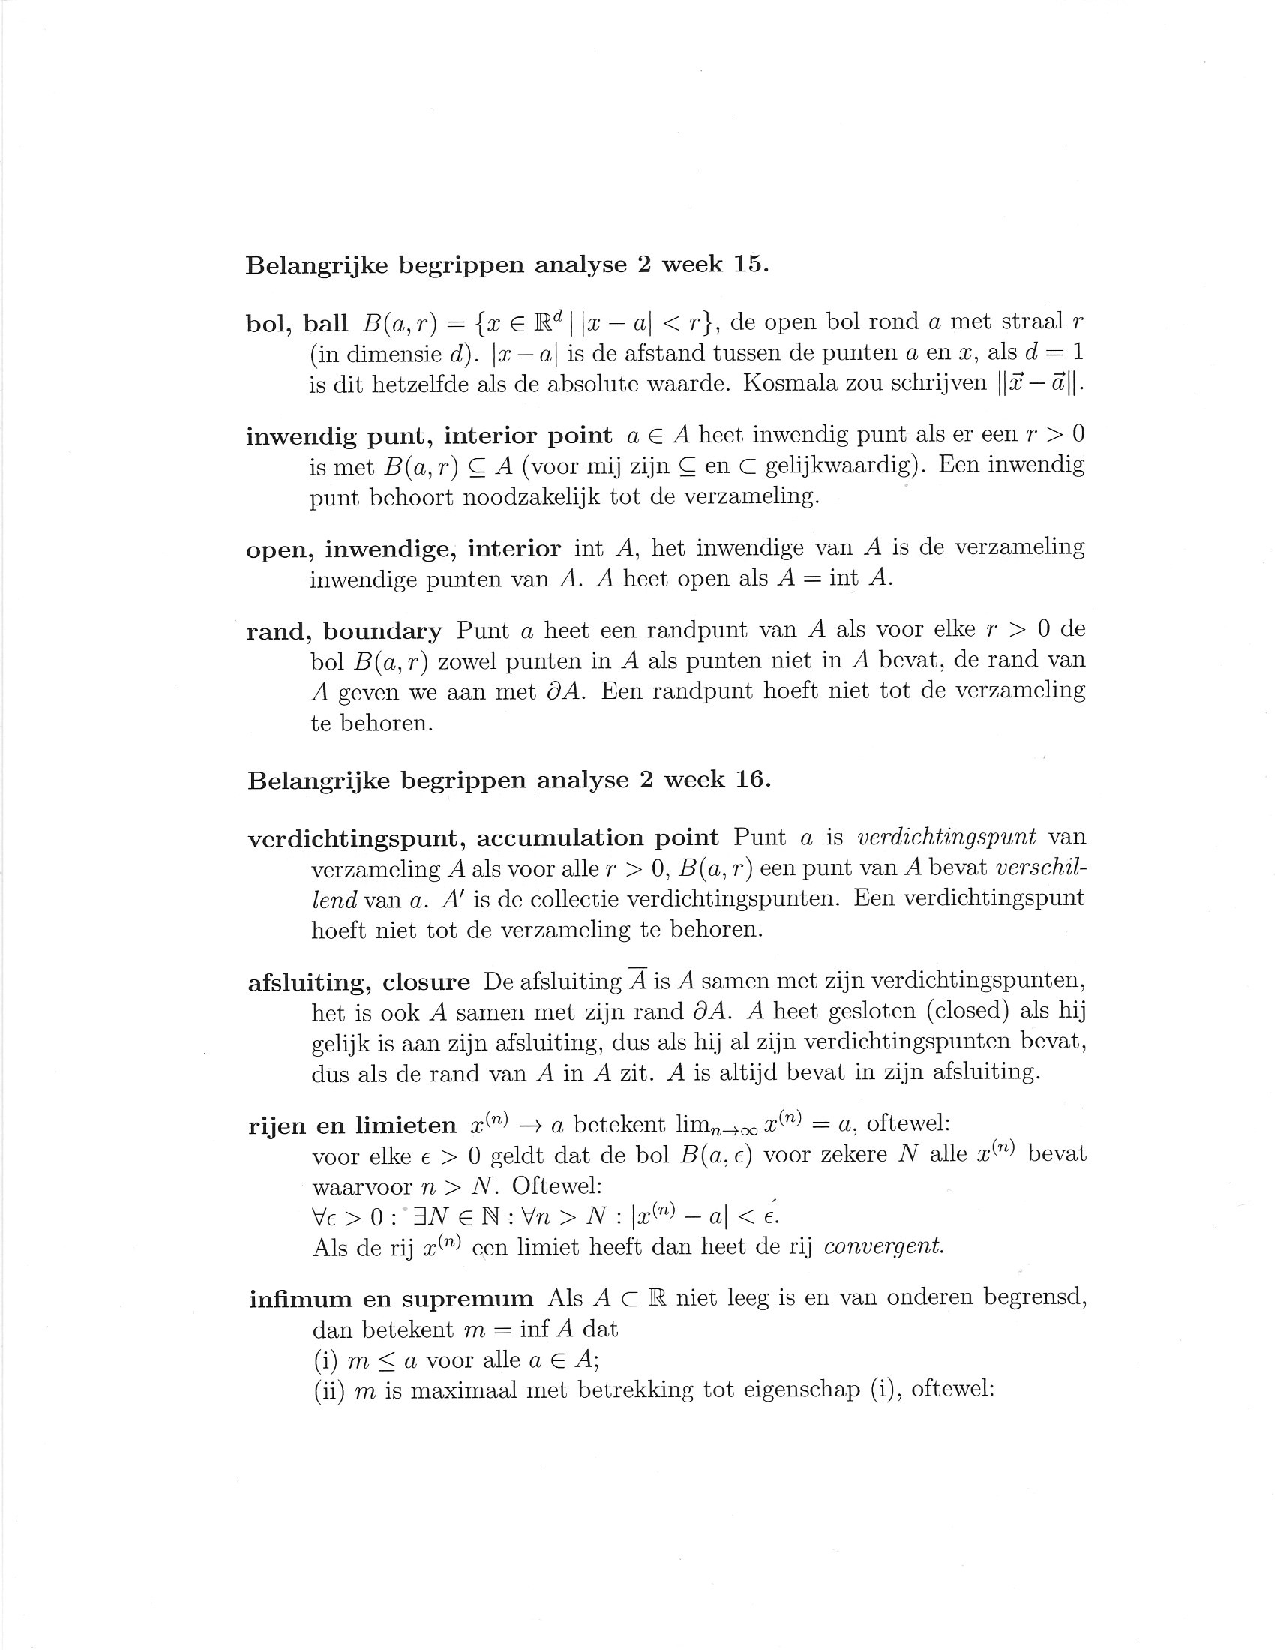
\includepdf[pages={-}]{Aart.pdf}
		
\end{document} 